\chapter{Computational study}
\label{chap:computational_study}
This chapter will give the most insights into the functionality and efficiency of the usage of the presented binary classifier in
\gls{3L-CVRP} algorithms. This chapter will begin with the selection of two different suiting \gls{3L-CVRP} datasets by comparing
several datasets and presenting the most important specialities. Afterwards the results from training the model are presented, which
is divided in three main parts, firstly the results of the retrieval of the data, secondly the feature selection, and finally presenting
different strategies for comparing different models and selecting the best regarding accuracy on the test dataset as well as on collected
tensor data. Afterwards a parameter study is conducted for the \gls{ILS}, starting with the \textit{NoClassifier} variant determining
the best configurations for the base parameters, followed by a more intense comparisons of all the classifier parameters determining the
other three variants. This chapter closes with a complete comparison of all four variants, comparing the version with tuned parameters.
These insights lay the foundation for the following closing Chapter~\ref{chap:conclusion}.

\section{Comparison of Available Datasets}
\label{sec:dataset_selection}

The \gls{3L-CVRP} is a well-studied problem and several datasets were published in the past, considering
different constraints and characteristics. A selection of these datasets will be compared and evaluated
in this section. The goal is to identify a suitable dataset for training a general \gls{CLP} classifier that can predict
the feasibility of the \gls{CLP} of single tours from different datasets. Therefore, the dataset needs
heterogeneous characterists to represent numerous possible use-cases
as shown in Chapter~\ref{sec:motivation_feasibility_prediction}. Five published
\cgls{3L-CVRP} datasets are presented with respect to their overall characteristics.
Each dataset gets an unique identfier to simplify the comparison and is shown in parenthesis
after the following individual introduction. The first \cgls{3L-CVRP} dataset was published by \citeauthor{gendreau_tabu_2006} in
\citeyear{gendreau_tabu_2006} and delivered the first \cgls{3L-CVRP} instances containing huge and heavy items (\gendreauDataSet).\footcite[cf.][]{gendreau_tabu_2006}
The second dataset was published by \citeauthor{moura_integrated_2009} in \citeyear{moura_integrated_2009},
and combines the \gls{VRP} from \citeauthor{solomon_algorithms_1987} and the \gls{CLP} instances from
\citeauthor{bischoff_issues_1995} defining the \gls{3L-VRPTW} considering
many items of small size and weight (\mouraDataSet).\footcites[cf.][]{solomon_algorithms_1987,bischoff_issues_1995}[][]{moura_integrated_2009}
The first dataset containing real-life data was published by \citeauthor{ceschia_local_2013} in \citeyear{ceschia_local_2013}
and contains the instances with the most items (\ceschiaDataSet).\footcite[cf.][]{ceschia_local_2013}
Krebs published two different datasets in
\citeyear{krebs_advanced_2021} with a focus on more realistic constraints. The first one contains a set
of realistic constraints and offers a wide range of instance sizes (\krebsADataSet).\footcite[cf.][]{krebs_advanced_2021}
The second one focuses on semi-trailer trucks and special requirements for axle weights (\krebsBDataSet).\footcite[cf.][]{krebs_axle_2021}
The characteristics of the datasets are summarized in the following Table~\ref{tab:dataset_comparison},
where the brackets [\,] indicate a range of possible values. All values considering mass and volume are
\textit{relative} to the respective vehicle weight and volume limit to be comparable. A \textit{item type} is
defined by its geometrical dimensions, the weight, and possible stability characteristics, such as fragility or \gls{LBS}.
When the number of item types is smaller than the number of items, items with equal type occur multiple times. The item types
depict the number of different item types per instance. Additionaly
most features of the dataset are compared with \textit{aggregated}  values, referring to the aggregrated characteristics
of all items requested by one customer, so the aggregated mass, volume and items shows the value what is requested by an
average customer of this dataset.

\newcolumntype{C}[1]{>{\centering\arraybackslash}p{#1}}
\newcolumntype{L}[1]{>{\raggedright\arraybackslash}p{#1}} % left-aligned
\begin{table}[ht]
    \centering
    \small
    \renewcommand{\arraystretch}{1.1}   % a touch more row height
    \begin{tabular}{@{}lccccc@{}}
        \toprule
        \textbf{Dataset} & \textbf{Instances} & \textbf{Customers} & \textbf{Agg. Mass}\footnote{Average is based on all customers of the instances.} & \textbf{Agg. Vol.} \footnotemark[\value{footnote}]       & \textbf{Agg. Items}\footnotemark[\value{footnote}] \\
        \midrule
        \gendreauDataSet & 27                 & [15, 100]          & 0.137                                                                            & 0.127                                                    & 2.00                                               \\
        \mouraDataSet    & 46                 & 25                 & 0.077                                                                            & 0.176                                                    & 52.0                                               \\
        \ceschiaDataSet  & 13                 & [11, 129]          & 0.063                                                                            & 0.160                                                    & 18.1                                               \\
        \krebsADataSet   & 600                & [20, 100]          & 0.098                                                                            & 0.100                                                    & 4.41                                               \\
        \krebsBDataSet   & 80                 & [30, 120]          & 0.036                                                                            & 0.052                                                    & 4.00                                               \\
        \toprule
        \textbf{Dataset} & \textbf{Items}     & \textbf{Types}     & \textbf{\text{Routes}}\footnote{Average is based on the instances.}              & \textbf{\text{Route Len}}\footnotemark[\value{footnote}] & \textbf{Fragility}\footnotemark[\value{footnote}]  \\
        \midrule
        \gendreauDataSet & [26, 199]          & [26, 199]          & 6.13                                                                             & 6.22                                                     & 0.25                                               \\
        \mouraDataSet    & 1050, 1550         & 5                  & 4.40                                                                             & 6.72                                                     & 0.29                                               \\
        \ceschiaDataSet  & [254, 8060]        & [9, 97]            & 10.2                                                                             & 5.81                                                     & 0.10                                               \\
        \krebsADataSet   & 200, 400           & 3, 10, 100         & 6.77                                                                             & 13.6                                                     & 0.24                                               \\
        \krebsBDataSet   & 200, 400           & 10, 100            & 3.87                                                                             & 22.1                                                     & 0.10                                               \\
        \bottomrule
    \end{tabular}
    \caption[Numerical comparison of different 3L--CVRP Datasets.]{Numeric comparisons between five avalaible datasets.}
    \label{tab:dataset_comparison}
\end{table}

The values routes, route length and fragility show the average over all instances, and
routes define the \gls{LB} for needed vehicles and route lenght the \gls{UB} for the customers in a route based on the average
requested relative volume and mass. The averages are displayed to become a better understanding of the average
statistics of each dataset, rather than looking at extreme values.
The most important consideration, when selecting a suitable dataset for the training of a classifier,
is how representative single tours from one dataset are for all other datasets. Therefore, the numeric characteristics
should not contain outliers. It is apparent, that the \gendreauDataSetText dataset has the least items per customer
with huge relative volume and weight values, which leads with an average route length of 6.22 customers to very few items
considered per route in comparison to the other datasets. This makes it easier to compute the feasibility of the laoding
as the number of placing patterns is limited. The \mouraDataSetText has the most items per average per customer consisting
of only 5 item types. The \ceschiaDataSetText dataset contains the fewest instances, but with the most maximum items of 8060,
which lead to many routes on avrage with average length and many items per loading. The two datasets from Krebs, have similar
boundaries and values, but \krebsBDataSetText has routes with twice as many customers as \krebsADataSetText on average due
to the smaller average aggregated mass and volume requested by each customer. Both \krebsADataSetText and \gendreauDataSetText
show a good variety of the features, without including too many items per route in comparison to the other datasets.
The following Table~\ref{tab:constraint_matrix} provides an overview of the constraints considered
in each dataset showcasing the realistic profile. The constraints are categorized in the five groups introduced
in Section~\ref{sec:clp_definition}.
\clearpage

\begin{table}[ht]
    \centering
    \small
    \renewcommand{\arraystretch}{1.2}
    \begin{tabular}{@{}L{1.8cm}L{3cm}C{1.6cm}C{1.6cm}C{1.6cm}C{1.6cm}C{1.6cm}@{}}
        \toprule
        \textbf{Category}          & \textbf{Constraint} &                        &                     & \textbf{Dataset}      &                      &                      \\
                                   &                     & Gendreau\newline(2006) & Moura\newline(2009) & Ceschia\newline(2013) & Krebs\newline(2021a) & Krebs\newline(2021b) \\
        \midrule
        \multirow{3}{*}{Container} & Load Capacity       & $\bullet$              & $\bullet$           & $\bullet$             & $\bullet$            & $\bullet$            \\
                                   & Load Balance        &                        &                     &                       & $\bullet$            &                      \\
                                   & Axle Weights        &                        &                     &                       & $\bullet$            & $\bullet$            \\\midrule
        \multirow{3}{*}{Item}      & z-Rotation          & $\bullet$              & $\bullet$           & $\bullet$             & $\bullet$            & $\bullet$            \\
                                   & Fragility           & $\bullet$              &                     & $\bullet$             & $\bullet$            & $\bullet$            \\
                                   & LBS                 &                        &                     & $\bullet$             & $\bullet$            &                      \\\midrule
        \multirow{1}{*}{Cargo}     & Complete Shipm.     & $\bullet$              & $\bullet$           &                       & $\bullet$            & $\bullet$            \\\midrule
        \multirow{6}{*}{Position}  & Geometry            & $\bullet$              & $\bullet$           & $\bullet$             & $\bullet$            & $\bullet$            \\
                                   & Orthogonality       & $\bullet$              & $\bullet$           & $\bullet$             & $\bullet$            & $\bullet$            \\
                                   & Reachability        &                        &                     & $\bullet$             & $\bullet$            &                      \\
                                   & Sequence            & $\bullet$              &                     &                       & $\bullet$            &                      \\
                                   & LIFO                & $\bullet$              & $\bullet$           & $\bullet$             & $\bullet$            & $\bullet$            \\
                                   & MLIFO               &                        &                     & $\bullet$             & $\bullet$            &                      \\\midrule
        \multirow{2}{*}{Load}      & Robust Stability    &                        &                     & $\bullet$             & $\bullet$            &                      \\
                                   & Support Area        & $\bullet$              & $\bullet$           &                       &                      & $\bullet$            \\

        \bottomrule
    \end{tabular}
    \caption[Overview of CLP constraints in selected 3L--CVRP datasets.]{Matrix overview of constraints covered in selected datasets. A bullet ($\bullet$) indicates that the constraint is considered.}
    \label{tab:constraint_matrix}
\end{table}

This comparison shows that all datasets include similar types of constraints, but the level
of complexity varies. \krebsADataSetText and \ceschiaDataSetText stand out by incorporating
more advanced constraints such as robust stability, reachability, and \gls{LBS}, in comparison to
basic ones like support area, \gls{LIFO} and fragility. To further investigate the differences
between the datasets, Figure~\ref{fig:dataset_comparison} visualizes the aggregated relative mass and
volume of all items requested by individual customers.
Additionally, the size of each scatter point indicates the total number of items requested.
For example, the \mouraDataSetText dataset includes 46
instances with 25 customers each, resulting in $25 \cdot 46 = 1150$ dots in the plot.

\begin{figure}[ht]
    \centering
    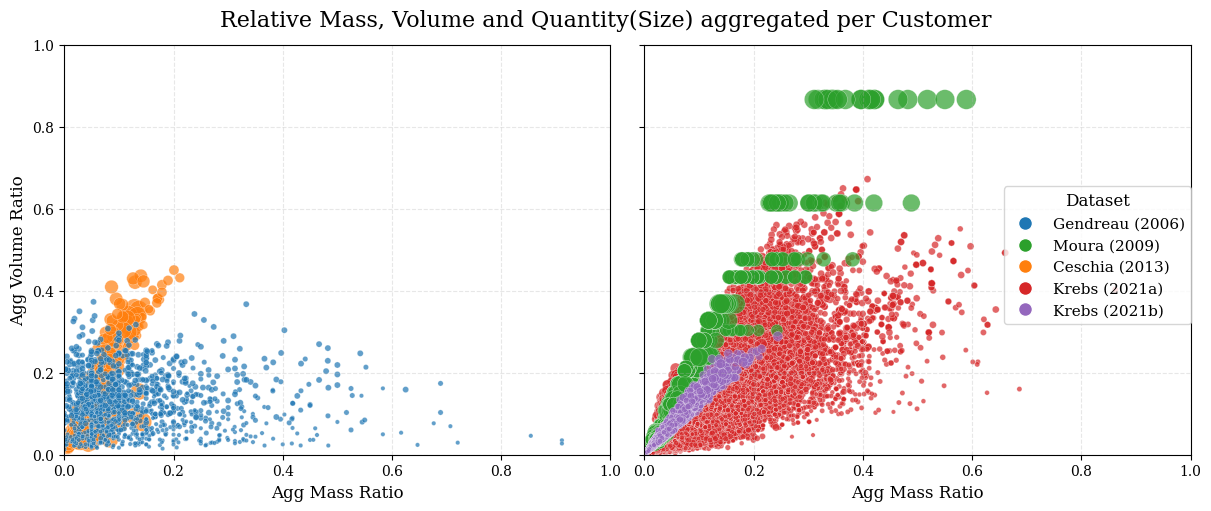
\includegraphics[width=0.85\textwidth]{pictures/comparison_datasets_3lcvrp.png}
    \caption{Comparison aggregated customer demands of different 3L--CVRP/ 3L--VRPTW datasets.}
    \label{fig:dataset_comparison}
\end{figure}

The dispersion of the data points reflects the diversity of individual instances in terms of volume
and mass dependency. A more balanced profile suggests that some customers tend to order items that
are either mass- or volume-intensive, which supports training the model on more heterogeneous data.
Therefore, the dataset should cover a wide range of cases, varying in mass, volume, and item
quantity per customer. The widest spread is observed in \krebsADataSetText and \gendreauDataSetText serving
both as good dataset candidates for training a classifier. Both datasets are investigated further in
the next section.

\section{Analsis of datasets}
\label{sec:analysis_datasets}

The two datasets, \krebsADataSetText and \gendreauDataSetText, have a good diverse profile for training
a binary classifier and to be further analyzed. It must be noted, that it is very likely more complex
to solve instances from the \krebsADataSetText as the number of customers in a route and the
aggregated number of items is on average twice as high as from \gendreauDataSetText (see Table~\ref{tab:dataset_comparison}).
As shown in Section~\ref{sec:literature_overview} several publications solved the Gendreau instance set
with various heuristics and even exact approaches, whereas only one heuristic solution approach exists for the instances of Krebs.
Both datasets are further analysed in this section to understand dataset specific properties, which could not
be shown in the previous section.

\subsubsection{\krebsADataSetText}

The dataset contains 18 different instance types resulting from the combinations
of number of customers, item types and items. The following Figure~\ref{fig:krebs_dataset_analysis_detailes} plots
the relative mass and volume of all items requested by individual customers for each of the 18 instances. Every color
represents one instance and the plots are divided by the number of respective customers in threee groups, presenting
6 combinations each. There are three levels for the different item types per [3,10,100] and two levels for the total
number of items, 200 and 400, per instance.

\begin{figure}[ht]
    \centering
    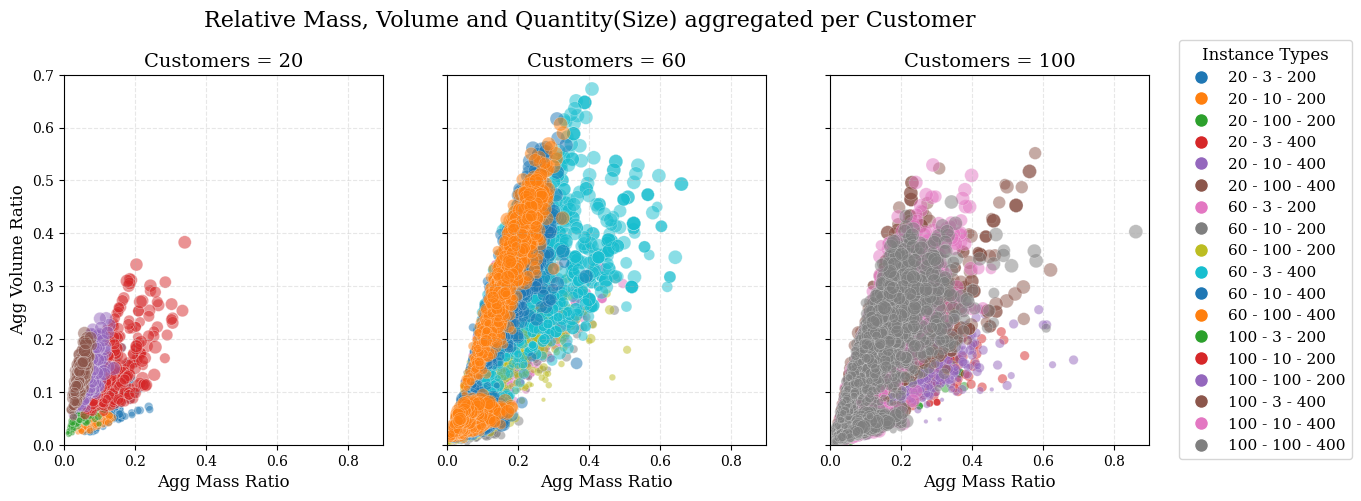
\includegraphics[width=0.85\textwidth]{pictures/krebs_instances_detailed.png}
    \caption[Visualization of different instances of \textcite{krebs_advanced_2021} dataset.]{Visualization of different instances of \krebsADataSetText dataset.
        The instances are named by the number of customers, item types and items.}
    \label{fig:krebs_dataset_analysis_detailes}
\end{figure}

Several insights can be obtained from the analysis of this plot. Firstly, the aggregated relative
volume and mass per customer is significantly lower for the 20 customers group than for the groups with 60 or 100 customers.
Secondly, the distribution differs from each instance type, ranging from quite linear distributions in a narrow
interval (e.g. instance 60-100-400) to quite broad distributions (e.g. instance 100-100-400). These two observations need to be considered,
when selecting instances to generate training data for the classifier to avoid a homogenous training set, and
as a consequence poor classifying results with a low accuracy. The instance set should be drawn from every group equally and
different distributions need to be considered per group, that the average route numeric route structure differs.

\subsubsection{\gendreauDataSetText}

This dataset consists of 27 instances, where the dispersion of the aggregated mass per customer is reaching very high values, up to
0.91, but has modest volume levels, with a maximum of 0.4 approximately, as could be seen in Figure~\ref{fig:dataset_comparison}. The
following Figure~\ref{fig:aggregated_gendreau_plots} show this dispersion per instance revealing an important insight about the dataset.
As the relative volume is quite for all instances, the relative mass differs between the instances. As it was analyzed from \cite{tamke_branch-and-cut_2024}
the complexity to solve the instances is far greater, when the items are more lightweight and the volume is the limiting factor
for packing items in the container. Furthermore, the authors distinguished the instances in a group of heavy items ($\mathcal{H}$) and
a group of lighweight items ($\mathcal{L}$) by dividing the two groups by the average weight utilization $\overline{\omega}$ of the found
groups. If $\overline{\omega} \geq 0.7$ then an instance belongs to $\mathcal{H}$ and for values smaller than 0.7 to $\mathcal{L}$.\footcite[cf.][pp. 23-25]{tamke_branch-and-cut_2024}
The obtained resutls for the Gendreau instances will be also differentiated in those two groups to investigate the effect of
the average weight utilization $\overline{\omega}$ on the solution quality and process.

\begin{figure}[ht]
    \centering
    \begin{tikzpicture}[node distance=0mm and 0mm]
        \node[anchor=south, inner sep=0] (A) at (0,0)
        {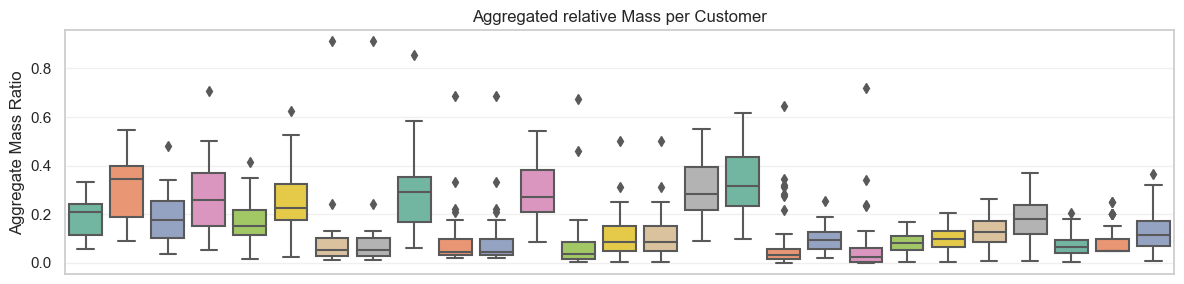
\includegraphics[width=0.95\textwidth]{pictures/AggMassCustGendreau.png}};
        \node[anchor=north, below=of A,inner sep=0] (B)
        {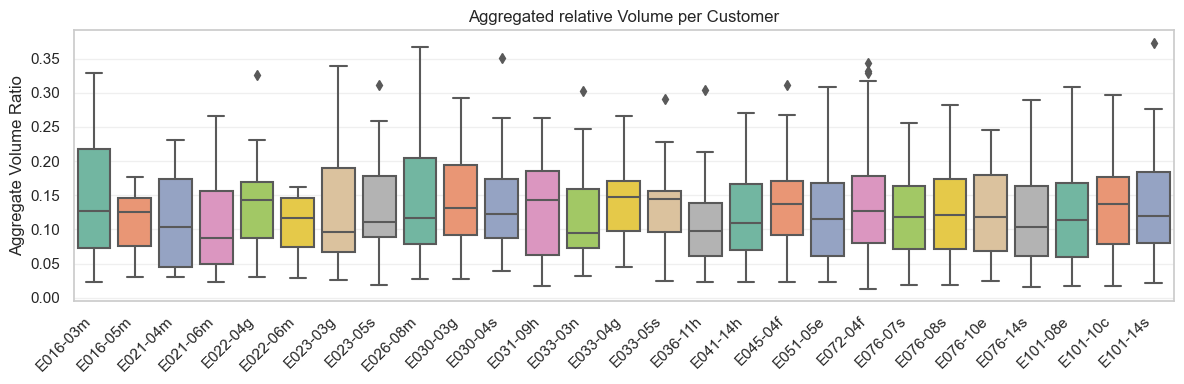
\includegraphics[width=0.96\textwidth]{pictures/AggVolCustGendreau.png}};
    \end{tikzpicture}
    \caption{Aggregated relative mass and volume per customer distributed for each instance of the \gendreauDataSetText dataset.}
    \label{fig:aggregated_gendreau_plots}
\end{figure}

In the following section the results from training the binary classifier are presented with diffferent datasets.

\section{Results Training}
\label{sec:ResultsTraining}
In this section the results from the feature dataset selection are discussed. The single best features
with individual scores are shown in the Appendix~\ref{app:feature_selection}. For each model variant (see Section~\ref{sec:modelselection})
the most suiting dataset is selected from both, the Random Retrieval and Save Strategy datasets. These selected
models will then be used in the further steps of the computational study to compare the \gls{ILS} algorithm
with and without the boost of the classifier. The tables where the single \gls{ML} variants are compared
can also be found in the appendix and this section can be reduced to present the datasets for each
retrieval strategy, as well as the final outcomes.

\subsection{Random Retrieval Strategy}
With the algorithm \ref{alg:rand_routes_generation} the following random datasets were created with all
instances from Gendreau.
\begin{table}[h!]
    \centering
    \begin{tabular}{@{}P{0.13\textwidth}P{0.08\textwidth}P{0.08\textwidth}P{0.08\textwidth}P{0.09\textwidth}P{0.10\textwidth}P{0.12\textwidth}P{0.12\textwidth}@{}}
        \midrule
        Name       & $\alpha$ & $\beta$ & $\gamma$ & Routes & Balance & Rel. Vol & Rel. Mass \\
        \bottomrule
        RD-2-20-20 & 2        & 20      & 20       & 45733  & 60/40   &          &           \\
        RD-2-20-30 & 2        & 20      & 30       & 70067  & 60/40   &          &           \\
        RD-2-30-20 & 2        & 30      & 20       & 47350  & 60/40   &          &           \\
        RD-2-30-30 & 2        & 30      & 30       & 72408  & 60/40   &          &           \\
        RD-3-20-20 & 3        & 20      & 20       & 68506  & 60/40   &          &           \\
        RD-3-20-30 & 3        & 20      & 30       & 104967 & 60/40   &          &           \\
        RD-3-30-20 & 3        & 30      & 20       & 70843  & 60/40   &          &           \\
        RD-3-30-30 & 3        & 30      & 30       & 108597 & 60/40   &          &           \\
        RD-4-20-20 & 4        & 20      & 20       & 91000  & 60/40   &          &           \\
        RD-4-20-30 & 4        & 20      & 30       & 139996 & 60/40   &          &           \\
        RD-4-30-20 & 4        & 30      & 20       & 94666  & 60/40   &          &           \\
        RD-4-30-30 & 4        & 30      & 30       & 144311 & 60/40   &          &           \\
        RD-5-40-40 & 5        & 40      & 40       & 249762 & 60/40   &          &           \\
        \bottomrule
    \end{tabular}
    \caption[Created instances for different parameter combinations $(\alpha, \beta, \gamma)$ for \gendreauDataSetText dataset.]{Created instances for different parameter combinations $(\alpha, \beta, \gamma)$ for \gendreauDataSetText dataset.
        The values in the balance column stand for the share of positive and netative labels in the sample population. The relative volume
        and mass refer to the average value for all routes in the respective dataset.}
    \label{tab:created_instances_xyz_gendreau}
\end{table}

\subsubsection{Save Retrieval Strategy}
The initial routes saved are from this and that dataset, it was tested if modificaions to reduce
the number of routes with 2 customers, lead to better model results. Therefore it was tested
to shrink all feasible routes with 2 customers with a similarity of $94\%$(Shrinked) or alternatively drop
all feasible routes with 2 customers (Trimmed). The three resulting datasets have the following characterics:

\begin{table}[ht]
    \centering
    \begin{tabular}{c c c c c}
        \toprule
        Name     & Routes & Balance & Rel. Vol & Rel. Mass \\
        \midrule
        Complete & 7616   & 60/40   &          &           \\
        Trimmed  & 15948  & 60/40   &          &           \\
        Shrinked & 24573  & 60/40   &          &           \\
        \bottomrule
    \end{tabular}
    \caption[Save strategy train datsets from \gendreauDataSetText.]{Save strategy train datsets from \gendreauDataSetText.
        The values in the balance column stand for the share of positive and netative labels in the sample population. The relative volume
        and mass refer to the average value for all routes in the respective dataset.}
    \label{tab:saved_instances_gendreau}
\end{table}

For the upcoming parameter study the following datasets were selected for the corresponding models
to analyse the performance of the classifier. It can be observed, that in general the ... datasets
do have more influence.

\begin{table}[ht]
    \centering
    \begin{tabular}{c c c c c c c}
        \toprule
        Model                          & Strategy & Name       & \gls{MCC}-Score & \gls{AUROC} & F1-Score & Accuracy \\
        \midrule
        \multirow{2}{*}{\gls{LR}}      & Random   & RD-4-20-30 & 0.6             & 0.87        & 0.9      & 0.8      \\
                                       & Save     & Complete   & 0.6             & 0.87        & 0.9      & 0.8      \\
        \midrule
        \multirow{2}{*}{Decision Tree} & Random   & RD-4-20-30 & 0.6             & 0.87        & 0.9      & 0.8      \\
                                       & Save     & Complete   & 0.6             & 0.87        & 0.9      & 0.8      \\
        \midrule
        \multirow{2}{*}{\gls{FFNN}}    & Random   & RD-4-20-30 & 0.6             & 0.87        & 0.9      & 0.8      \\
                                       & Save     & Complete   & 0.6             & 0.87        & 0.9      & 0.8      \\

        \bottomrule
    \end{tabular}
    \caption{Presentatione of final datasets and feature selection}
    \label{tab:final_dataset_features}
\end{table}

\section{Parameter Study}
\label{sec:parameter_study}

The parameter study is divided in four subsections following the variants of the algorithm
presented in Section~\ref{sec:FeasibilityCheck}. This study follows a hierarchical procedure
tuning the parameters, introduced for each variant, sequentially. The following subset of instances
from the gendreau dataset is used:

\begin{itemize}
    \item E016-03m
    \item E030-03g
    \item ...
\end{itemize}

The division followed the following approach, first all instances were omitted, which found
the optimal solution (see \cite{tamke_branch-and-cut_2024}\footcite[cf.][p.26]{tamke_branch-and-cut_2024})
in a short time. Second, similar instances of size and complexity were reduced to only one.
Every instance is run three times with different seeds and a timelimit of 10min. It will be investigated
how different parameter combinations influence the RDP, the iteration number, the rejection rate and
the average improvement per second after finding the initial solution.

\subsection{NoClassifier Variant}
\label{subsec_parameterStuy_noclassifier}
For this variant all the basic \gls{ILS} paramters will be tested as this displays the base form
for all the upcoming variants, but with the limitation, that the loading is only checked
with the exact \gls{CP} solver.
The following variations were tested and the resulting box plots are showed afterwards and
will be analyed afterwards.


\begin{table}[ht]
    \centering
    \begin{tabular}{c c }
        \toprule
        Parametertype      & Levels                             \\
        \midrule
        AttemptsLimit      & [3,5,8,12]                         \\
        RoundLimit         & [1,5,8]                            \\
        RandomMoves K      & [3,5,8]                            \\
        BasePerturbation   & [K-RandomSwaps,K-RandomInsertions] \\
        Neighborhood order & [IntraFirst, InterFirst]           \\
        \bottomrule
    \end{tabular}
    \caption{Parameter levels for NoClassifier variant.}
    \label{tab:parameters_noclassifier}
\end{table}

\subsection{SpeedUp Variant}
\label{subsec_parameterStuy_speedup}

\begin{table}[ht]
    \centering
    \begin{tabular}{c c }
        \toprule
        Parametertype            & Levels     \\
        \midrule
        IterationsWithoutCPCheck & [1,3,5,10] \\
        UseFilterStartSolution   & [1,0]      \\
        \bottomrule
    \end{tabular}
    \caption{Parameter levels for SpeedUp variant.}
    \label{tab:parameters_speedup}
\end{table}

\subsection{Hybrid Variant}
\label{subsec_parameterStuy_hybrid}

\begin{table}[ht]
    \centering
    \begin{tabular}{c c }
        \toprule
        Parametertype             & Levels                      \\
        \midrule
        Hybrid Usage Alternatives & \{[1,1,0],[1,0,1],[0,1,1]\} \\
        UseFilterStartSolution    & [1,0]                       \\
        \bottomrule
    \end{tabular}
    \caption{Parameter levels for hybrid variant.}
    \label{tab:parameters_hybrid}
\end{table}